% Document/LinearAlgebra/VectorSpaces/Foundations/MinkowskiSum.tex
% Section: Minkowski Structure on P(V)

\newpage
\section{Minkowski Structure on $\mathcal{P}(V)$}

\begin{definition}[Minkowski Sum]\label{def:minkowski-sum}
    Let $V$ be a $K$-vector space and $A, B \subseteq V$. The \textbf{Minkowski sum} of $A$ and $B$ is
    \[
        \MinkowskiSum{A}{B} = \Set{a + b \mid a \in A, b \in B}
    \]
\end{definition}

\begin{example}[Minkowski Sum Examples]\label{ex:minkowski-sum}
    Consider the following examples:
    \begin{enumerate}
        \item In $\bb{R}$: $\MinkowskiSum{\{1,2\}}{\{10,20\}} = \{11, 21, 12, 22\}$
        \item In $\bb{R}$: $\MinkowskiSum{[0,1]}{[0,1]} = [0,2]$
        \item In $\bb{R}^2$: If $L$ is a line through the origin and $p$ is a point, then
              $\MinkowskiSum{L}{\{p\}}$ is a line parallel to $L$ passing through $p$.
    \end{enumerate}

    \begin{center}
    \begin{tikzpicture}[scale=0.8, >=stealth]
        % Line through origin
        \draw[thick, blue] (-2,-1) -- (2,1) node[right] {$L$};
        \fill[blue] (0,0) circle (2pt) node[below left] {$0$};

        % Point p
        \fill[red] (1,2) circle (2pt) node[above] {$p$};

        % Translated line
        \draw[thick, purple, dashed] (-1,1) -- (3,3) node[right] {$L + \{p\}$};

        % Arrow showing translation
        \draw[->, gray, thick] (0,0) -- (1,2);
    \end{tikzpicture}
    \end{center}

    For singletons, we use the notation $\MinkowskiSum{u}{U} \defeq \MinkowskiSum{\{u\}}{U}$ (translation of $U$ by $u$).
\end{example}

\begin{definition}[Minkowski Scalar-Set Product]\label{def:minkowski-prod}
    Let $L \subseteq K$ and $A \subseteq V$. The \textbf{Minkowski scalar-set product} is
    \[
        \MinkowskiProd{L}{A} = \Set{\lambda a \mid \lambda \in L, a \in A}
    \]
\end{definition}

\begin{example}[Minkowski Product Examples]\label{ex:minkowski-prod}
    Consider the following examples:
    \begin{enumerate}
        \item In $\bb{R}$: $\MinkowskiProd{\{1,2\}}{\{3\}} = \{3, 6\}$
        \item In $\bb{R}$: $\MinkowskiProd{[0,1]}{[0,1]} = [0,1]$
        \item In $\bb{R}^n$: For $v \neq 0$, $\MinkowskiProd{\bb{R}}{\{v\}} = \Set{\lambda v \mid \lambda \in \bb{R}}$
              is the line through the origin in direction $v$.
    \end{enumerate}

    \begin{center}
    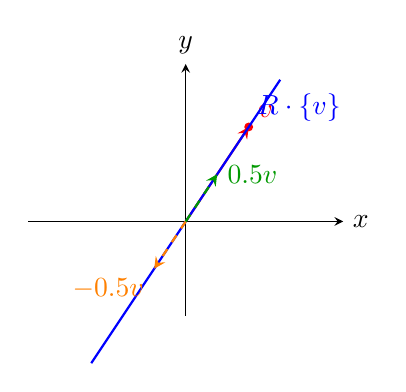
\begin{tikzpicture}[scale=0.8, >=stealth]
        % Axes
        \draw[->] (-2.5,0) -- (2.5,0) node[right] {$x$};
        \draw[->] (0,-1.5) -- (0,2.5) node[above] {$y$};

        % Vector v
        \fill[red] (1,1.5) circle (2pt) node[above right] {$v$};
        \draw[->, thick, red] (0,0) -- (1,1.5);

        % Line through origin = R*{v}
        \draw[thick, blue] (-1.5,-2.25) -- (1.5,2.25);
        \node[blue] at (1.8,1.8) {$\bb{R} \cdot \{v\}$};

        % Scaling indication
        \draw[->, thick, orange, dashed] (0,0) -- (-0.5,-0.75) node[below left] {$-0.5v$};
        \draw[->, thick, green!60!black, dashed] (0,0) -- (0.5,0.75) node[right] {$0.5v$};
    \end{tikzpicture}
    \end{center}

    For singletons, we write $\MinkowskiProd{\lambda}{A} \defeq \MinkowskiProd{\{\lambda\}}{A}$ (scalar multiplication of the set).
\end{example}

\begin{proposition}[Monoid Structure of $(\mathcal{P}(V), +)$]\label{prop:minkowski-monoid}
    The Minkowski sum satisfies:
    \begin{enumerate}
        \item \textbf{Associativity}: $(A + B) + C = A + (B + C)$
        \item \textbf{Commutativity}: $A + B = B + A$
        \item \textbf{Identity}: $\{0\} + A = A$
        \item \textbf{Absorbing element}: $\emptyset + A = \emptyset$
    \end{enumerate}
\end{proposition}

\begin{proof}
    Properties (1)--(3) follow directly from the corresponding axioms of vector addition.
    For (4), note that $\emptyset + A = \Set{a + b \mid a \in \emptyset, b \in A} = \emptyset$
    since there are no elements in $\emptyset$.
\end{proof}

\begin{proposition}[Monoid Action of $(\mathcal{P}(K), \cdot)$ on $\mathcal{P}(V)$]\label{prop:minkowski-action}
    The Minkowski scalar-set product satisfies:
    \begin{enumerate}
        \item \textbf{Identity}: $\{1_K\} \cdot A = A$
        \item \textbf{Compatibility}: $(L \cdot M) \cdot A = L \cdot (M \cdot A)$
        \item \textbf{Absorbing}: $\emptyset \cdot A = \emptyset$ and $L \cdot \emptyset = \emptyset$
        \item \textbf{Zero properties}: $L \cdot \{0\} = \{0\}$ if $L \neq \emptyset$;
              $\{0\} \cdot A = \{0\}$ if $A \neq \emptyset$
    \end{enumerate}
\end{proposition}

\begin{proof}
    (1) We have $\{1_K\} \cdot A = \Set{1_K \cdot a \mid a \in A} = \Set{a \mid a \in A} = A$.

    (2) Both sides equal $\Set{\lambda \mu a \mid \lambda \in L, \mu \in M, a \in A}$.

    (3) Follows from the empty set having no elements.

    (4) If $L \neq \emptyset$, then $L \cdot \{0\} = \Set{\lambda \cdot 0 \mid \lambda \in L} = \{0\}$.
    Similarly for $\{0\} \cdot A$.
\end{proof}

\begin{proposition}[Monotonicity]\label{prop:minkowski-monotone}
    Minkowski operations are monotone:
    \begin{enumerate}
        \item If $A \subseteq B$, then $A + C \subseteq B + C$
        \item If $A \subseteq B$, then $LA \subseteq LB$
        \item If $L \subseteq M$, then $LA \subseteq MA$
    \end{enumerate}
\end{proposition}

\begin{proof}
    Each property follows immediately: elements of the LHS are also elements of the RHS
    since $A \subseteq B$ or $L \subseteq M$.
\end{proof}

\begin{proposition}[Partial Distributivity]\label{prop:partial-distrib}
    For all $L, M \subseteq K$ and $A, B \subseteq V$:
    \begin{enumerate}
        \item $L(A + B) \subseteq LA + LB$
        \item $(L + M)A \subseteq LA + MA$
    \end{enumerate}
\end{proposition}

\begin{proof}
    (1) Let $x \in L(A + B)$. Then $x = \lambda(a + b)$ for some $\lambda \in L$, $a \in A$, $b \in B$.
    By distributivity in $V$: $x = \lambda a + \lambda b \in LA + LB$.

    (2) Let $x \in (L + M)A$. Then $x = (\lambda + \mu)a$ for some $\lambda \in L$, $\mu \in M$, $a \in A$.
    By distributivity in $V$: $x = \lambda a + \mu a \in LA + MA$.
\end{proof}

\begin{example}[Failure of Reverse Inclusions]\label{ex:distrib-failure}
    The reverse inclusions of Proposition~\ref{prop:partial-distrib} do not hold in general:
    \begin{enumerate}
        \item $LA + LB \not\subseteq L(A + B)$: Take $L = \{1, 2\}$, $A = B = \{1\}$ in $\bb{R}$.
              Then $L(A + B) = \{1, 2\} \cdot \{2\} = \{2, 4\}$, but
              $LA + LB = \{1, 2\} + \{1, 2\} = \{2, 3, 4\}$.
              We have $3 \in LA + LB$ but $3 \notin L(A + B)$.

        \item $LA + MA \not\subseteq (L + M)A$: Take $L = M = \{1\}$, $A = \{0, 1\}$ in $\bb{R}$.
              Then $(L + M)A = \{2\} \cdot \{0, 1\} = \{0, 2\}$, but
              $LA + MA = \{0, 1\} + \{0, 1\} = \{0, 1, 2\}$.
              We have $1 \in LA + MA$ but $1 \notin (L + M)A$.
    \end{enumerate}
\end{example}

\begin{proposition}[Full Distributivity Conditions]\label{prop:full-distrib}
    The reverse inclusions hold under these conditions:
    \begin{enumerate}
        \item If $L = \{\lambda\}$ is a singleton, then $\lambda A + \lambda B = \lambda(A + B)$
        \item If $A = \{a\}$ is a singleton, then $La + Ma = (L + M)a$
        \item If $KB = B$ and $0 \in A$, then $LA + LB = L(A + B)$
        \item If $KA = A$, $A + A = A$, and $L + M \neq \{0\}$, then $LA + MA = (L + M)A$
    \end{enumerate}
\end{proposition}

\begin{proof}
    (1) Let $x \in \lambda A + \lambda B$, so $x = \lambda a + \lambda b$ for some $a \in A$, $b \in B$.
    Then $x = \lambda(a + b) \in \lambda(A + B)$.

    (2) Let $x \in La + Ma$, so $x = \lambda a + \mu a$ for some $\lambda \in L$, $\mu \in M$.
    Then $x = (\lambda + \mu)a \in (L + M)a$.

    (3) Assume $KB = B$ and $0 \in A$. Let $x = \lambda a + \mu b \in LA + LB$.

    \textit{Case $\lambda \neq 0$}: Since $KB = B$, we have $(\mu/\lambda)b \in B$.
    Thus $x = \lambda(a + (\mu/\lambda)b) \in L(A + B)$.

    \textit{Case $\lambda = 0$}: Then $x = \mu b = \mu(0 + b) \in L(A + B)$ since $0 \in A$.

    (4) Assume $KA = A$, $A + A = A$, $L + M \neq \{0\}$. Let $x = \lambda a + \mu a' \in LA + MA$.

    \textit{Case $\lambda + \mu \neq 0$}: Since $KA = A$ and $A + A = A$,
    $\frac{\lambda}{\lambda+\mu}a + \frac{\mu}{\lambda+\mu}a' \in A$.
    Thus $x = (\lambda + \mu) \cdot \left(\frac{\lambda}{\lambda+\mu}a + \frac{\mu}{\lambda+\mu}a'\right) \in (L + M)A$.

    \textit{Case $\lambda + \mu = 0$}: Then $\mu = -\lambda$ and $x = \lambda(a - a')$.
    Since $L + M \neq \{0\}$, there exist $\lambda' \in L$, $\mu' \in M$ with $\lambda' + \mu' \neq 0$.
    Since $KA = A$ and $A + A = A$, we have $\frac{\lambda}{\lambda' + \mu'}(a - a') \in A$.
    Thus $x = (\lambda' + \mu') \cdot \frac{\lambda}{\lambda' + \mu'}(a - a') \in (L + M)A$.
\end{proof}

\begin{proposition}[Distributivity over Unions]\label{prop:union-distrib}
    For arbitrary families:
    \begin{enumerate}
        \item $A + \BigUnion[i \in I] B_i = \BigUnion[i \in I] (A + B_i)$
        \item $L \cdot \BigUnion[i \in I] A_i = \BigUnion[i \in I] LA_i$
        \item $\left(\BigUnion[i \in I] L_i\right) \cdot A = \BigUnion[i \in I] L_i A$
    \end{enumerate}
\end{proposition}

\begin{proof}
    (1) We have $x \in A + \BigUnion[i \in I] B_i$ iff $x = a + b$ with $a \in A$ and $b \in B_j$ for some $j$,
    iff $x \in A + B_j$ for some $j$, iff $x \in \BigUnion[i \in I] (A + B_i)$.

    (2) and (3) are analogous.
\end{proof}

\begin{proposition}[Sub-Distributivity over Intersections]\label{prop:intersect-subdistrib}
    For arbitrary families:
    \begin{enumerate}
        \item $A + \BigIntersect[i \in I] B_i \subseteq \BigIntersect[i \in I] (A + B_i)$
        \item $L \cdot \BigIntersect[i \in I] A_i \subseteq \BigIntersect[i \in I] LA_i$
        \item $\left(\BigIntersect[i \in I] L_i\right) \cdot A \subseteq \BigIntersect[i \in I] L_i A$
    \end{enumerate}
\end{proposition}

\begin{proof}
    (1) If $b \in \BigIntersect[i \in I] B_i$, then $b \in B_i$ for all $i$,
    so $a + b \in A + B_i$ for all $i$, hence $a + b \in \BigIntersect[i \in I] (A + B_i)$.
\end{proof}

\begin{example}[Counterexamples for Reverse Intersection Inclusions]\label{ex:intersect-failure}
    The reverse inclusions fail:
    \begin{enumerate}
        \item $(A + B) \Intersect (A + C) \not\subseteq A + (B \Intersect C)$:
              Take $A = \{0, 1\}$, $B = \{0\}$, $C = \{1\}$ in $\bb{R}$.
              Then $B \Intersect C = \emptyset$, so $A + (B \Intersect C) = \emptyset$.
              But $(A + B) \Intersect (A + C) = \{0, 1\} \Intersect \{1, 2\} = \{1\} \neq \emptyset$.

        \item $LA \Intersect LB \not\subseteq L(A \Intersect B)$:
              Take $L = \{1, 2\}$, $A = \{1\}$, $B = \{2\}$ in $\bb{R}$.
              Then $A \Intersect B = \emptyset$, so $L(A \Intersect B) = \emptyset$.
              But $LA \Intersect LB = \{1, 2\} \Intersect \{2, 4\} = \{2\} \neq \emptyset$.
    \end{enumerate}
\end{example}

\begin{proposition}[Singleton Equality for Intersections]\label{prop:singleton-intersect}
    For singletons:
    \begin{enumerate}
        \item $\{a\} + \BigIntersect[i \in I] B_i = \BigIntersect[i \in I] (\{a\} + B_i)$
        \item $\{\lambda\} \cdot \BigIntersect[i \in I] A_i = \BigIntersect[i \in I] \{\lambda\} A_i$
    \end{enumerate}
\end{proposition}

\begin{proof}
    (1) If $x \in \BigIntersect[i \in I] (\{a\} + B_i)$, then for each $i$, $x = a + b_i$ for some $b_i \in B_i$.
    But $b_i = x - a$ is the same for all $i$, so $x - a \in \BigIntersect[i \in I] B_i$,
    hence $x \in \{a\} + \BigIntersect[i \in I] B_i$.

    (2) is analogous (for $\lambda \neq 0$; if $\lambda = 0$, both sides equal $\{0\}$).
\end{proof}
